\documentclass[letterpaper]{article}
\usepackage[margin=1in]{geometry}
\usepackage[utf8]{inputenc}
\usepackage{textcomp}
\usepackage{amssymb}
\usepackage{natbib}
\usepackage{graphicx}
\usepackage{gensymb}
\usepackage{amsthm, amsmath, mathtools}
\usepackage[dvipsnames]{xcolor}
\usepackage{enumerate}
\usepackage{mdframed}
\usepackage[most]{tcolorbox}
\usepackage{csquotes}
% https://tex.stackexchange.com/questions/13506/how-to-continue-the-framed-text-box-on-multiple-pages

\tcbuselibrary{theorems}

\newcommand{\R}{\mathbb{R}}
\newcommand{\Z}{\mathbb{Z}}
\newcommand{\N}{\mathbb{N}}
\newcommand{\Q}{\mathbb{Q}}
\newcommand{\C}{\mathbb{C}}
\newcommand{\code}[1]{\texttt{#1}}
\newcommand{\mdiamond}{$\diamondsuit$}
\newcommand{\PowerSet}{\mathcal{P}}
\newcommand{\Mod}[1]{\ (\mathrm{mod}\ #1)}
\DeclareMathOperator{\lcm}{lcm}

%\newtheorem*{theorem}{Theorem}
%\newtheorem*{definition}{Definition}
%\newtheorem*{corollary}{Corollary}
%\newtheorem*{lemma}{Lemma}
\newtheorem*{proposition}{Proposition}


\newtcbtheorem[number within=section]{theorem}{Theorem}
{colback=green!5,colframe=green!35!black,fonttitle=\bfseries}{th}

\newtcbtheorem[number within=section]{definition}{Definition}
{colback=blue!5,colframe=blue!35!black,fonttitle=\bfseries}{def}

\newtcbtheorem[number within=section]{corollary}{Corollary}
{colback=yellow!5,colframe=yellow!35!black,fonttitle=\bfseries}{cor}

\newtcbtheorem[number within=section]{lemma}{Lemma}
{colback=red!5,colframe=red!35!black,fonttitle=\bfseries}{lem}

\newtcbtheorem[number within=section]{example}{Example}
{colback=white!5,colframe=white!35!black,fonttitle=\bfseries}{def}

\newtcbtheorem[number within=section]{note}{Important Note}{
        enhanced,
        sharp corners,
        attach boxed title to top left={
            xshift=-1mm,
            yshift=-5mm,
            yshifttext=-1mm
        },
        top=1.5em,
        colback=white,
        colframe=black,
        fonttitle=\bfseries,
        boxed title style={
            sharp corners,
            size=small,
            colback=red!75!black,
            colframe=red!75!black,
        } 
    }{impnote}
\usepackage[utf8]{inputenc}
\usepackage[english]{babel}
\usepackage{fancyhdr}
\usepackage[hidelinks]{hyperref}

\pagestyle{fancy}
\fancyhf{}
\rhead{CSE 130}
\chead{Monday, April 25, 2022}
\lhead{Lecture 13}
\rfoot{\thepage}

\setlength{\parindent}{0pt}

\begin{document}
\section{Representing Complex Data}
\subsection{Recursive Types}
Let's define \textbf{natural numbers} from scratch; in particular,
\begin{verbatim}
    data Nat = Zero | Succ Nat \end{verbatim}
Specifically, a \code{Nat} is either 
\begin{itemize}
    \item An empty box labeled \code{Zero},
    \item or a box labeled \code{Succ} with another \code{Nat} in it.
\end{itemize}
Some examples of \code{Nat} values are 
\begin{verbatim}
    Zero                                        -- 0
    Succ Zero                                   -- 1
    Succ (Succ Zero)                            -- 2
    Succ (Succ (Succ Zero))                     -- 3
\end{verbatim}

\subsubsection{Functions on Recursive Types}
We can then write a recursive function for this type:
\begin{verbatim}
    data Nat = Zero             -- Base Constructor
                | Succ Nat      -- Inductive Constructor \end{verbatim}
Call this function \code{toInt}, which convers the recursive type to its corresponding number. First, we add a pattern for each constructor. 
\begin{verbatim}
    toInt :: Nat -> Int 
    toInt Zero      = ...       -- Base Case 
    toInt (Succ n)  = ...       -- Inductive Case (Recursive Call Goes Here) \end{verbatim}
Next, we can fill in the base case.
\begin{verbatim}
    toInt :: Nat -> Int 
    toInt Zero      = 0
    toInt (Succ n)  = ...\end{verbatim}
After that, we can fill in the inductive case using a recursive step.
\begin{verbatim}
    toInt :: Nat -> Int 
    toInt Zero      = 0
    toInt (Succ n)  = 1 + toInt n\end{verbatim}

\begin{mdframed}[]
    (Quiz.) What does this evaluate to? 
    \begin{verbatim}
        let foo i = if i <= 0 then Zero else Succ (foo (i - 1))
        in foo 2 \end{verbatim}    
    \begin{enumerate}[(a)]
        \item Syntax error
        \item Type error 
        \item \code{2}
        \item \code{Succ Zero}
        \item \code{Succ (Succ Zero)}
    \end{enumerate}

    \begin{mdframed}[]
        The answer is \textbf{E}. This function does the reverse of \code{toInt}; that is, given an \code{Int}, it returns the \code{Nat} representation. 
    \end{mdframed}
\end{mdframed}

\subsubsection{Recursive Type as Result}
TODO 


\subsubsection{Putting the Two Together}
Let us now implement the \code{add} function.
\begin{verbatim}
    add :: Nat -> Nat -> Nat 
    add Zero        m = m               -- Base Case 
    add (Succ n')   m = Succ (add n' m) -- Inductive Case \end{verbatim}
The idea is that $n' = n - 1$, so we're basically doing $n - 1 + m$ for the \code{add} function in the inductive case. What we want is $n + m$, so we can use \code{Succ} to add one. 

\bigskip

Subtraction is somewhat more difficult.
\begin{verbatim}
    sub :: Nat -> Nat -> Nat 
    sub n           Zero        = n
    sub Zero        _           = Zero 
    sub (Succ n')   (Succ m')  = sub n' m' 
\end{verbatim}
Here, we have that $n' = n - 1$ and $m' = m - 1$, so we're doing $n - 1 - (m - 1) = n - 1 - m + 1 = n - m$. 

\subsection{Lists}
Note that lists are not built-in. In fact, they are an algebraic data type like any other. So,
\begin{verbatim}
    data List = Nil 
                | Cons Int List 
\end{verbatim}
So, \code{[1, 2, 3]} is represented by \code{Cons 1 (Cons 2 (Cons 3 Nill))}. So, we can think of the built-in list constructors \code{[]} and \code{(:)} as fancy syntax for \code{Nil} and \code{Cons}.

\bigskip 

Functions on lists follow the same general strategy. For example, 
\begin{verbatim}
    length :: List -> Int 
    length Nil          = 0
    length (Cons _ xs)  = 1 + length xs \end{verbatim}

What about \code{append}ing two lists? 
\begin{verbatim}
    append :: List -> List -> List 
    append xs ys = ??\end{verbatim}
One implementation is 
\begin{verbatim}
    append :: List -> List -> List 
    append Nil          ys  = ys 
    append (Cons x xs)  ys  = Cons x (append xs ys)\end{verbatim}
Now, we expect \code{append [1, 2] [3, 4]} to give us \code{[1, 2, 3, 4]}. Indeed, this is the expected result that we get.

\subsection{Calculator}
Suppose you want to implement an arithmetic calculator to evaluate expressions like 
\begin{itemize}
    \item \code{4.0 + 2.9}
    \item \code{3.78 - 5.92}
    \item \code{(4.0 + 2.9) * (3.78 - 5.92)}
\end{itemize}
What is a datatype that we can use to represent these expressions? 
\begin{verbatim}
    data Expr = Num Float 
                | Add Expr Expr 
                | Sub Expr Expr 
                | Mul Expr Expr\end{verbatim}

Now, how do we write said function to evaluate an expression?
\begin{verbatim}
    eval :: Expr -> Float 
    eval (Num x)        = x
    eval (Add e1 e2)    = (eval e1) + (eval e2)
    eval (Sub e1 e2)    = (eval e1) - (eval e2)
    eval (Mul e1 e2)    = (eval e1) * (eval e2)
\end{verbatim}


\subsection{Trees}
We can think of lists as \emph{unary trees}. 
\begin{verbatim}
     Cons 
      1  
        \
         \ 
          \ 
          Cons 
           2
             \ 
              \ 
               \ 
               Nil 
\end{verbatim}

In particular, we can represent lists using the following datatype:
\begin{verbatim}
    data List = Null | Cons Int List\end{verbatim}
How do we represent binary trees? Generally, a binary tree is just a bunch of nodes that can either have more nodes or leaves. 

\begin{mdframed}[]
    (Quiz.) What is a Haskell datatype that can represent this binary tree?
    \begin{center}
        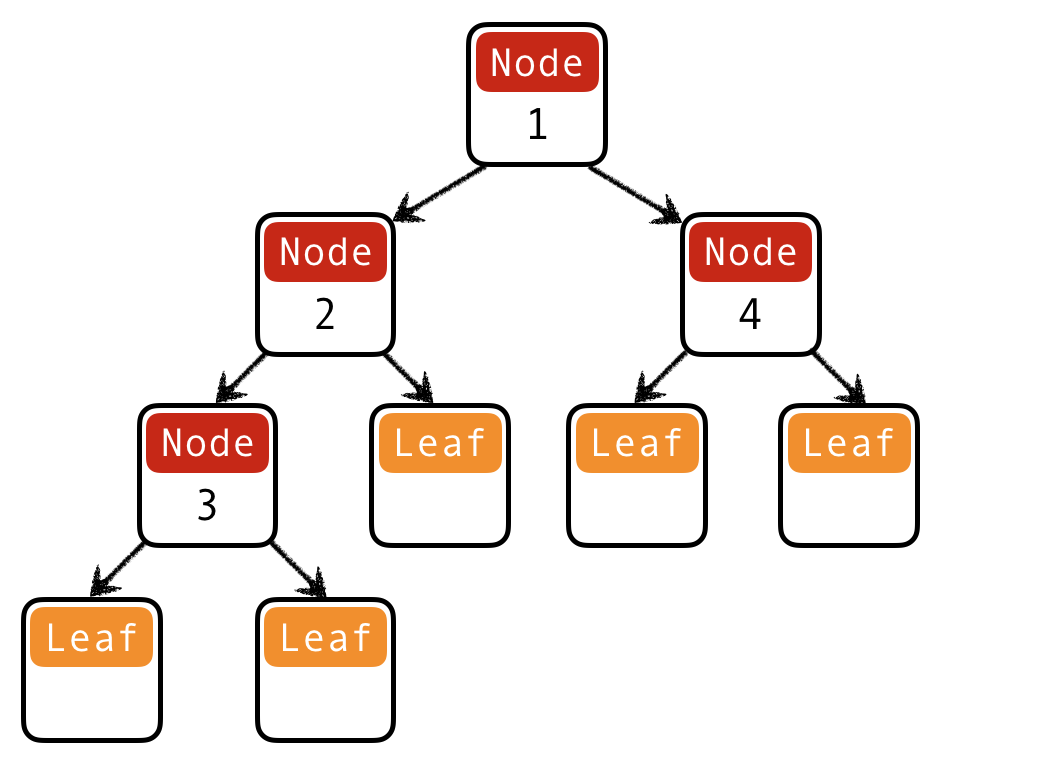
\includegraphics[scale=0.4]{../assets/tree-data-node.png}
    \end{center}

    \begin{enumerate}[(a)]
        \item \code{data Tree = Leaf | Node Int Tree}
        \item \code{data Tree = Leaf | Node Tree Tree}
        \item \code{data Tree = Leaf | Node Int Tree Tree}
        \item \code{data Tree = Leaf Int | Node Tree Tree}
        \item \code{data Tree = Leaf Int | Node Int Tree Tree}
    \end{enumerate}

    \begin{mdframed}[]
        The answer is \textbf{C}. Note that each \code{Node} has an \code{Int} value associated with it, but each \code{Leaf} doesn't. Also note that each \code{Node} -- which has two \code{Tree}s, hence the name -- can just be a \code{Leaf}.
    \end{mdframed}
\end{mdframed}

\end{document}